\section{Introdução}

De uma maneira geral, uma \textdef{função} é uma ferramenta matemática utilizada para relacionar dois conjuntos quaisquer. A relação é feita mapeando cada elemento de um conjunto à \emph{exatamente um} elemento do outro conjunto.

\begin{example}
Para entender melhor, considere dois conjuntos $X$ e $Y$ e assuma que existem $x \in X$ e $y \in Y$. Sendo assim, podemos mapear o objeto $x$ ao objeto $y$ através de uma função $f$. Isto é, ao aplicarmos a função $f$ em $x$, obtemos $y$. Para expressar essa afirmação utilizamos a notação $f(x) = y$. E podemos interpretar como na imagem a seguir:

\begin{center}
     \tikzset{every picture/.style={line width=0.75pt}} %set default line width to 0.75pt        

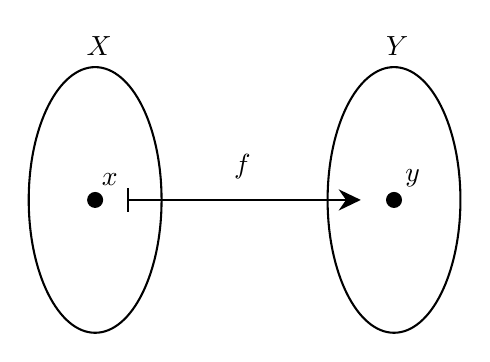
\begin{tikzpicture}[x=0.75pt,y=0.75pt,yscale=-1,xscale=1]
%uncomment if require: \path (0,308); %set diagram left start at 0, and has height of 308

%Shape: Ellipse [id:dp8584080168945698] 
\draw   (160,112) .. controls (160,76.65) and (174.33,48) .. (192,48) .. controls (209.67,48) and (224,76.65) .. (224,112) .. controls (224,147.35) and (209.67,176) .. (192,176) .. controls (174.33,176) and (160,147.35) .. (160,112) -- cycle ;
%Straight Lines [id:da9209150729175881] 
\draw    (192,112) ;

\draw [shift={(192,112)}, rotate = 0] [color={rgb, 255:red, 0; green, 0; blue, 0 }  ][fill={rgb, 255:red, 0; green, 0; blue, 0 }  ][line width=0.75]      (0, 0) circle [x radius= 3.35, y radius= 3.35]   ;
%Straight Lines [id:da7784202535308219] 
\draw    (336,112) ;

\draw [shift={(336,112)}, rotate = 0] [color={rgb, 255:red, 0; green, 0; blue, 0 }  ][fill={rgb, 255:red, 0; green, 0; blue, 0 }  ][line width=0.75]      (0, 0) circle [x radius= 3.35, y radius= 3.35]   ;
%Shape: Ellipse [id:dp3856498056795209] 
\draw   (304,112) .. controls (304,76.65) and (318.33,48) .. (336,48) .. controls (353.67,48) and (368,76.65) .. (368,112) .. controls (368,147.35) and (353.67,176) .. (336,176) .. controls (318.33,176) and (304,147.35) .. (304,112) -- cycle ;
%Straight Lines [id:da4011502733578831] 
\draw    (208,112) -- (318,112) ;
\draw [shift={(320,112)}, rotate = 180] [fill={rgb, 255:red, 0; green, 0; blue, 0 }  ][line width=0.75]  [draw opacity=0] (10.72,-5.15) -- (0,0) -- (10.72,5.15) -- (7.12,0) -- cycle    ;
\draw [shift={(208,112)}, rotate = 180] [color={rgb, 255:red, 0; green, 0; blue, 0 }  ][line width=0.75]    (0,5.59) -- (0,-5.59)   ;

% Text Node
\draw (263,96) node   {$f$};
% Text Node
\draw (199,102) node   {$x$};
% Text Node
\draw (194,38) node   {$X$};
% Text Node
\draw (337.5,38) node   {$Y$};
% Text Node
\draw (345,101.5) node   {$y$};

\end{tikzpicture}
\end{center}
\end{example}

Na imagem podemos ver que $X$ e $Y$ são conjuntos, $x \in X$ e $y \in Y$, e que $f(x) = y$, que daí temos $f(x) \in Y$.